\documentclass{thesis-ekf}
\usepackage[T1]{fontenc}
\PassOptionsToPackage{defaults=hu-min}{magyar.ldf}
\usepackage[magyar]{babel}
\usepackage{graphicx}
\usepackage{floatrow}
\usepackage{hyperref}
\usepackage{tocbibind}
\usepackage{url}
\def\UrlBreaks{\do\/\do-}
\usepackage{listingsutf8,xcolor,caption,multicol, subcaption, adjustbox}

\begin{document}
	\institute{Matematikai és Informatikai Intézet}
	\title{Mobil alkalmazás fejlesztés android platformon}
	\author{Nyeste Réka\\Programtervező informatikus BSc}
	\supervisor{Dr. Tajti Tibor Gábor\\Egyetemi docens}
	\city{Eger}
	\date{2024}
	\maketitle
	\tableofcontents
	\chapter*{Bevezetés}
	Azért választottam ezt a témát szakdolgozatomnak, mert szerintem fontos az, hogy a kezdő programozók megfelelő alapokat kapjanak a fejlődésük érdekében. Továbbiakban alkalmazásomat, a Codojo applikációt fogom bemutatni részletesen.
	
	Egyetemen folytatott tanulmányaim során számos tantárggyal és technológiával sikerült megismerkednem és tudásomat mélyítenem, azonban a mobil applikációkat találtam a legérdekesebbnek mind közül. Számomra ugyanis ígéretes az Android Studio azon tulajdonsága, hogy egy üres Activity-hez azonnal hozzárendel egy kinézetet, ami XML alapú és így a Backend résszel együtt tudom tervezni a Frontend részét is, rendkívül kényelmes és hatékony a fejlesztés szempontjából.
	
	A Codojo applikáció egy olyan alkalmazás, ami azon alapszik, hogy a felhasználó mennyire értette és tanulta meg a benne lévő tananyagot. Kétféle programozási nyelvről készítettem tanulnivalókat, illetve majdnem mindegyik anyagrész végén van egy néhány kérdésből álló teszt, a fejezetek végén pedig egy összefoglaló kérdéssorozat található, ami természetesen nem csak egy témát dolgoz fel, hanem az egész tananyagot. A kvízeket úgy állítottam össze, hogy összhangban maradjanak az elolvasott és megtanult programozós témákkal, ezt rendkívül fontosnak tartottam a fejlesztés során, hogy csak olyan kérdést tegyek fel, ami benne volt a tananyagban.
	
	Programozni tanulni véleményem szerint nem könnyű elkezdeni és még nehezebb folytatni is azt. Ezt az igényt kielégítve szerettem volna egy olyan alkalmazást fejleszteni, ami egy kicsit megkönnyíti a tanulási folyamatot és biztos alapot ad azoknak, akik úgy döntöttek, hogy szeretnének belekóstolni ebbe a remek szakmába. 
	
	\textit{A forráskódom megtekinthető ezen a linken: \url{https://github.com/rekanyeste/Codojo}}
	
	\chapter{Az alkalmazás tervezése}
	A szakdolgozatom megtervezése kezdetén nagy hangsúlyt fektettem a az applikáció nevére, mely nem véletlenül kapta a Codojo nevet. Szívügyemnek érzem azt, hogy aki belevág a programozásba az egy olyan biztos alapot, egy megfelelő háttértudást kapjon, hogy mire eljut a nehezebb témákig például az objektum-orientált programozás vagy alapelvek megismerése, annak ne okozzon semmilyen problémát ezeknek az elsajátítása. A Codojo-t a Code és Dojo szavakból alkottam meg, melynek Dojo része a japán harcművészetre, a karatére utal, jelentése: edzőterem. Nem véletlenül, hiszen egy edzőteremben is keményen kell dolgozni, valamint a kitartás és szorgalmasság is elengedhetetlen a kívánt eredmények elérése érdekében.
	\section{Android Studio}
	Korszerű, integrált környezetet biztosít szakdolgozatom számára. Könnyű benne dolgozni és remekül szétválasztható a Frontend és Backend fejlesztése. Ebben a fejlesztői környezetben két nyelv közül választhatunk: Java vagy Kotlin. Az applikációm számára a Java nyelvet választottam, hiszen egyetemi tanulmányaim során ebben mélyítettem el tudásomat.
	
	Az Android Studio a hivatalos integrált fejlesztői környezete (IDE) az Android alapú applikációknak. Az IntelliJ IDEA-hoz hasonlóan egy remek kódszerkesztő, illetve az alábbi fejlesztői eszközök is rendelkezésünkre állnak, hogy hatékonyságunkat növeljék:
	\begin{itemize}
		\item Rugalmas Gradle-alapú buildelési rendszer
		\item Gyors és részletgazdag emulátor
		\item Egységes környezet az összes Android eszköz fejlesztésére
		\item Emulátorok és fizikai készülékek valós idejű frissítésére szolgáló Live Edit
		\item Széleskörű tesztelési eszközök és keretrendszerek \cite{android_studio}
	\end{itemize}
	\section{Firebase}
	A Firebase a Google egy terméke, mely nagy segítsége a programozóknak alkalmazásaik fejlesztésében és kezelésében. Segítségével a fejlesztők gyorsabban és biztonságosabban készíthetik el az appokat. Firebase oldalon egyáltalán nem kell programozni, ez jelentősen megkönnyíti funkcióinak használatát. Androiddal, IOS-szel, weboldalakkal és Unity-vel is használható, valamint felhő alapú tárolást is biztosít. 
	
	Kezdetben nem Firebase volt a neve, hanem Envolve és online chates felületként indult. Fejlesztők ezt a felületet arra használták, hogy alkalmazások adatait, például játékok valós idejű állapotát, megosszák felhasználóikkal, tehát nem csevegésre. Ez szétválasztotta az Envolve-ot és a chatrendszert. James Tamplin és Andrew Lee, az  alapítók, fejlesztették tovább 2012-ben.
	\cite{firebase}
	\subsection{Firebase Realtime Database}
	Firebase ezen adatbázisa lehetőséget nyújt valós idejű adatok tárolására, mint például a bejelentkezés, regisztráció. Ez egy NoSQL alapú adatbázis, ami felhőben tárolja a felhasználók adatait azután is, hogy kiléptünk az alkalmazásból. HTTPS kérésekkel ellentétben adatszinkronizációt használ, ezzel lehetővé teszi, hogy ha például a felhasználó meg szeretné változtatni az egyik eltárolt adatát, akkor ezt pillanatokon belül megtegye. 
	
	A valós idejű adatbázis lehetőséget nyújt a fejlesztők számára, hogy olyan összetett alkalmazásokat írjanak, melyek biztonságos kapcsolatot tudnak létesíteni az adatbázissal közvetlenül a kliens oldali kódból. Offline állapotban is megtartják az eltárolt adatokat egy darabig, ezáltal sokkal jobb felhasználói élményt nyújtanak. Mikor ismét online lesz a felhasználó szinkronizálódnak az adatok és az esetlegesen bekövetkezett változások az adatbázisban automatikusan megjelennek.
	\cite{firebase_realtime}
	\subsection{Firebase Authentication}
	A Firebase-ben van egy különálló szolgáltatás csak az autentikációra. A Firebase Autentikáció támogatja a sima email + jelszó párossal a bejelentkezést (OAuth2 segítségével), de ezen felül még támogatja a Facebook, Google, Twitter és GitHub bejelentkezést. A különféle közösségi média platform bejelentkezés támogatásával meg tudjuk növelni a felhasználók számát, mivel sokkal egyszerűbb az átlag felhasználóknak így bejelentkezni.\cite{firebase_auth} A Codojo applikációban ezt a részt csak a kijelentkezésnél valósítom meg, mivel úgy döntöttem, hogy számomra és a felhasználók számára elegendő lesz a valós idejű adatbázis használata is.
	\section{GitHub}
	A Git-et 2005-ben Linus Torvalds fejlesztette ki nyílt forráskódú szoftverként, hogy nyomon követhesse a változásokat egy elosztott verziókezelő rendszerben.
	
	A Git egy verziókezelő rendszer, amely kezeli és nyomon követi a kódodat. A GitHub viszont egy szolgáltatás, amely lehetővé teszi a kód fájljainak hostolását, megosztását és kezelését az interneten.
	
	A Git és GitHub olyan népszerű eszközök, amelyeket a programozásban használnak. Segítenek abban, hogy különböző verzióit kezelni lehessen a kódnak és lehetővé tegye az együttműködést a fejlesztők között. A változásokat egy elosztott verziókezelő rendszeren keresztül követi. Ez azt jelenti, hogy követni tudja a projekt különböző verzióinak állapotát.
	
	A GitHub egy platform, ahol a Git felhasználók együtt építenek szoftvert. A GitHub emellett egy hosting szolgáltató és verziókezelő platform, amelyen nyílt forráskódú projekteken lehet együttműködni és fájlokat megosztani. \cite{github}
	
	\subsection{GitKraken}
	A GitKraken egy olyan eszköze a Git-nek, mely egy grafikus felhasználói felületet biztosít a programozók számára, ezzel segítve a közös munkát és a verziókövetést. Remek eszközeivel hatékonyan segíti a csapatmunkát például:
	\begin{itemize}
		\item beépített merge funkció,
		\item össze tud kapcsolódni a GitHub vagy Bitbucket fiókkal,
		\item könnyen alkalmazkodik a különböző környezetekhez és Gitflow támogatása van,
		\item gyorsbillentyűket is lehet használni. \cite{gitkraken}
	\end{itemize}
	
	Az Android Studio is támogatja a Git-et, ezzel a beépített funkcióval nagyszerűen nyomon tudtam követni a szakdolgozatom előrehaladását, valamint amennyiben vétettem benne hibát egyszerűen vissza tudtam keresni azt az állapotát a programnak, amelyikben még megfelelően működött és vissza tudtam azt állítani a hibamentes verzióra. Parancsai közül a Pull-t és Push-t használtam, melyekkel frissíteni volt lehetőségem a programomat egy újabb és jobb verzióra.
	
	\section{Android Emulátor}
	Ahhoz, hogy sikeresen futtatni lehessen egy Android Studioban megírt kódot, szükségem volt egy virtuális eszközre (Android Virtual Device). Ezt a projekt létrehozása után lehet konfigurálni. Én a Pixel virtuális telefont részesítettem előnyben, ami 30-as API szinttel van beállítva, így áthidalja azt a lehetséges hibát, hogy a felhasználó nem tudja futtatni a telefonján, mivel minél nagyobb API szintet állítok be, annál újabb eszközökön képes futni a program. A 30-as szint az Android 11-es verziót használja.
	
	\begin{figure}[tbh]
		\centering
		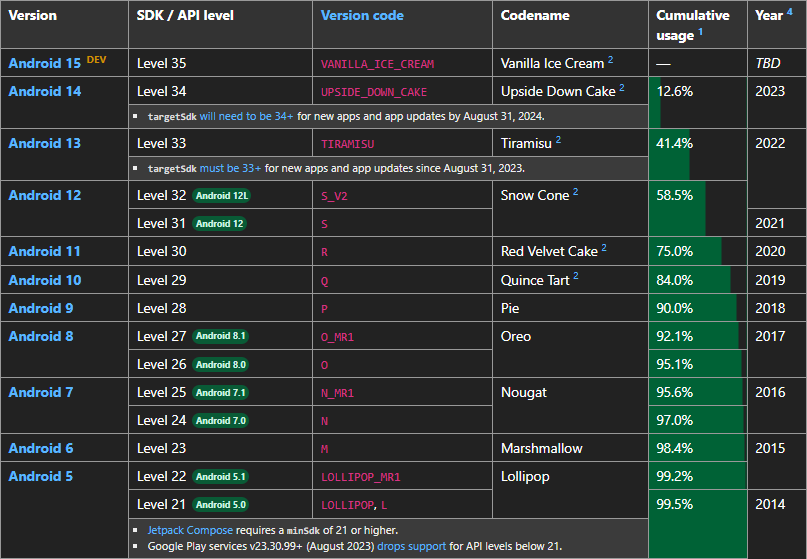
\includegraphics[width=1.0\linewidth]{api_szintek}
		\caption{API-szintek, forrás: \cite{api}}
		\label{apiszintek}
	\end{figure}
	
	\section{Java}
	Mobilapplikációt kétféle nyelven lehet megvalósítani Android Studioban: Kotlin és Java. Az utóbbit választottam, mivel több tantárgyam épült erre tanulmányaim során, ezért nem jelentett kihívást számomra, hogy szakdolgozatomat is ezen a nyelven írjam meg. Szakdolgozatom része az, hogy a kezdő programozókat, vagyis a felhasználókat bevezessem a Java világába, ezért az egyik tananyagomnak ezt választottam, melyben az alapokat könnyedén el tudják sajátítani.
	
	A Java egy rendkívül jól átvihető programozási nyelv, amelyet platformokon és különböző típusú eszközökön használnak, az okostelefonoktól az okostévékig. Többek között mobil- és webes alkalmazások, vállalati szoftverek, eszközök internetes hálózata (IoT), játékok, big data, elosztott és felhőalapú alkalmazások készítésére használják.
	
	A Java kódot először egy Java Development Kitben kell megírni, amely Windows, Linux és macOS operációs rendszerekhez érhető el. A programozók Java programozási nyelven írnak, melyet a készlet olyan számítógépes kóddá fordít, amelyet a megfelelő szoftverrel rendelkező bármely eszköz tud olvasni. Ez egy fordítónak nevezett szoftverrel érhető el. A fordító az olyan magas szintű számítógépes kódot, mint a Java, lefordítja egy olyan nyelvre, amelyet az operációs rendszerek értenek, és bájtkódnak neveznek. Ezután egy Java virtuális gépnek (JVM) nevezett értelmező dolgozza fel. A JVM-ek a legtöbb szoftver- és hardverplatformhoz elérhetők, és ez teszi lehetővé a Java-kód átvitelét egyik eszközről a másikra. Java futtatásához a JVM-ek betöltik a kódot, ellenőrzik azt, és futási környezetet biztosítanak. \cite{java}
	
	\section{Adatbázis tábla}
	Programomban a felhasználók regisztrációját, bejelentkezését és adatmódosítását a Users nevű táblában rögzítettem, melynek alapja a kódban lévő Users osztály, amelyet konstruktorokkal, valamint getter és setter metódusokkal láttam el.
	
	\begin{figure}[htb]
		\begin{floatrow}
			\ffigbox[\FBwidth]{\caption{Firebase Realtime Adatbázis}\label{adatbazisrealtime}}{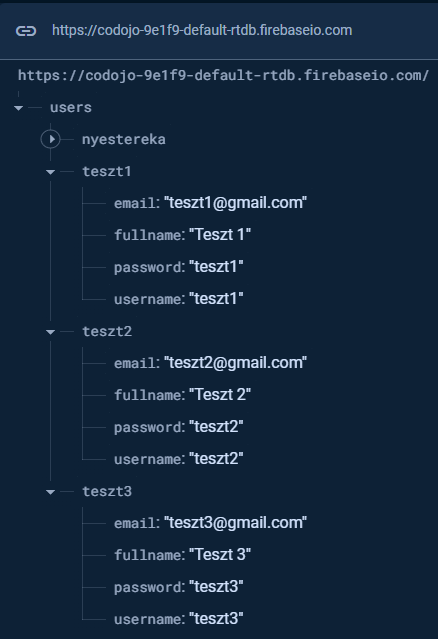
\includegraphics[width=1.1\linewidth]{adatbazis_realtime}}
		\end{floatrow}
	\end{figure}
	
	\section{Folyamatábra}
	A Codojo működését az alábbi folyamatábra szemlélteti:
	
	\begin{figure}[htb]
		\begin{floatrow}
			\ffigbox[\FBwidth]{\caption{Folyamatábra a program működéséről}\label{folyamatabra}}{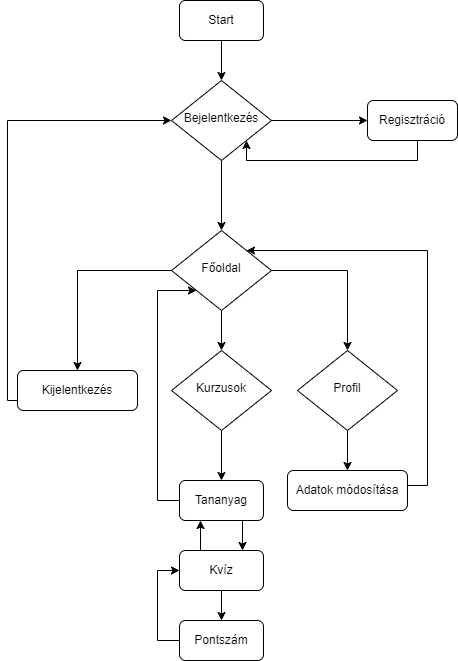
\includegraphics[width=1.2\linewidth]{folyamatabra}}
		\end{floatrow}
	\end{figure}

\chapter{Informatikaoktatás Magyarországon}
Bár egyre többen választanak informatikusképzést, még mindig hiányszakmának számít ez Magyarországon. Ennek oka, hogy sok iparág igényli a jól képzett informatikai szakembereket, a munkaerőpiaci kereslet rohamosan növekszik, amelyet azonban a kínálat kisebb tempóban követ.

Az informatikai szektor a nemzetgazdasági foglalkoztatás 4,1 százalékát, míg a versenyszféra 6,2 százalékát teszi ki. Az informatikusok havi bruttó átlagkeresete a második helyen áll a fizetések rangsorában.

Ezeket figyelembe véve nem meglepő, hogy a főiskolai és az egyetemi kereteken kívül számos tanfolyam és online képzés is elérhető az informatikai tudásra vágyók számára. A felsőoktatási intézmények alapképzésein gazdaságinformatikus, mérnökinformatikus, programtervező informatikus és üzemmérnök-informatikus képzéseken vehetünk részt. A mesterszakok között pedig az autonómrendszer-informatikus, a gazdaságinformatikus, mérnökinformatikus és a programtervező informatikus továbbképzések között válogathatunk.

\section{Gyakornoki programok szerepe}
Az informatikusképzésben résztvevők elmerülnek az analízis, a valószínűségszámítás, a lineáris algebra, az operációkutatás, a statisztika és a számítástudomány világában. Emellett megismerik azokat a természettudományi elveket, módszereket, amelyek nélkülözhetetlenek ahhoz, hogy jó szakember váljon belőlük. Megtanulják az informatikai rendszerek, a hardver és a szoftver elemeinek működését, valamint elsajátítják az informatikai rendszerek más rendszerekkel való összekapcsolásának képességét. A programtervező informatikusok a legfontosabb programozási elveket, programnyelveket és fejlesztési eszközöket is közelebbről tanulmányozzák.

Mivel az informatikusképzések összetett, széles körű területet ölelnek fel, a gyakornoki programok szerepe kulcsfontosságú. Sok esetben a cégek figyelik a kiemelkedő hallgatókat, és már az alapképzés után, a gyakornoki program során lecsapnak a legígéretesebb diákokra. Ez maga után vonja, hogy a tehetséges informatikusok nem feltétlenül folytatják tanulmányaikat mesterképzésen, hanem gyakornoki helyükön maradnak, ahol lehetőségük van gyakorlati tudásuk elmélyítésére. A felsőoktatási intézményekben túlnyomórészt elméleti oktatás folyik, azok a hallgatók, akiknek nem sikerül megfelelő gyakornoki helyet találniuk, gyakran hátrányba kerülnek társaikkal szemben.

\section{Gyakorlatorientált oktatás}
Két éve a Budapesti Műszaki és Gazdaságtudományi Egyetemen és a Pannon Egyetemen egy újfajta, gyakorlati oktatásra fókuszáló képzés indult: az üzemmérnök informatikus szak, amely felsőfokú alapképzést nyújt. A szak esetében kevesebb elméleti tárgy vár a hallgatókra, míg több gyakorlati órán, projektfeladatban és szakmai gyakorlaton kell részt venniük. Olyannyira gyakorlatorientált az oktatás, hogy a hároméves képzés utolsó évében már főként cégeknél gyakornoki munkát végeznek a hallgatók, hogy minél inkább elsajátíthassák a munkaerő piacon szükséges tudást.

A főiskolák és egyetemek mellett több felnőttoktatást kínáló intézményben is megjelentek az informatikai képzések, azonban a vállalatok magasan a felsőoktatásból kikerült diákokat preferálják. Az OKJ-s képzések minőségét, piaci értékét alacsonyra becsülik a piaci szereplők. Ezzel szemben azonban, akik a programozói hivatást szeretnék választani, nem feltétlenül kell, hogy a felsőoktatásban tanuljanak. A programozók számára kevésbé fontosak a természettudományos és matematikaelméleti ismeretek, így számukra jó megoldást kínálnak azok a tanfolyamok, amelyek elvégzésével gyakorlati programozói tudást szerezhetnek. A programozó képzések esetében a legtöbb vállalkozás nyitott a nem felsőoktatásban végzett hallgatók foglalkoztatására is.

\section{Nők szerepe az informatikában}
Az IVSZ – Szövetség a Digitális Gazdaságért kutatása alapján a legtöbb informatika iránt érdeklődő hallgató Budapesten folytatja tanulmányait. A fővárosi és vidéki intézmények fele-fele arányban képeznek ki informatikusokat. Egyre inkább igyekeznek bevonni a nőket is az informatikai képzésekbe, ám csupán 15 százalék körüli a nők aránya az informatikai alapszakokra felvettek esetében. A hölgyek körében legnépszerűbb a gazdaságinformatikus szak, ahol 28 százalékban képviselik magukat, a legkevésbé kedvelt pedig a mérnökinformatikus képzés, amely esetében csupán 9 százalék a nők aránya. Nem csak a felsőoktatási intézmények, de a cégek is támogatják a nők informatikai pályaválasztását elősegítő programokat. Sokan csupán a sztereotípiák miatt nem mernek jelentkezni, így már a középfokú intézményekben érdemes elkezdeni a nők informatikai pályaorientációjának elősegítését. Összességében a képzésben részt vevő hallgatók fele mérnökinformatikus szakon tanul, a legtöbb intézményben pedig elérhető a gazdaságinformatikus szak.

\section{Előnyt jelentene a nyelvtudás?}
Sok esetben a tehetséges, szenior pozíciókban dolgozó szakembereknek magasabb fizetést ajánlanak a külföldi cégek, és túlnyomórészt az informatikusok el is fogadják az ajánlatot. Különösen igaz ez a Z-generáció esetében, hiszen ők magasabb mobilitási hajlandósággal rendelkeznek, valamint angol nyelvtudásuk is erősebb. Itt érdemes megemlíteni, hogy azok a szakemberek, akik jól beszélik az angol nyelvet, hamarabb kapnak magas fizetéssel járó ajánlatot, mint azok, akiknek hiányosságaik akadnak ezen a téren. Nem csak abban az esetben lényeges a nyelvtudás, ha külföldön szeretnénk kamatoztatni informatikai tudásunkat, hanem akkor is, ha itthon szeretnénk egy multinacionális vállalatnál elhelyezkedni. Az angol nyelvtudás elengedhetetlen, ha érvényesülni szeretnénk a szakmában.

\section{Nyitottság az új dolgok felé}
A szakmai felkészültség és a nyelvtudás mellett azonban olyan készségekkel is rendelkezniük kell az informatikusoknak, mint a változásra való nyitottság, a jó problémamegoldó képesség, a kreativitás, a csapatban való dolgozás és a kiemelkedő kommunikációs érzék. A legtöbb felsőoktatási intézmény igyekszik ezeket a készségeket is átadni a hallgatóknak, hiszen a sikeres szakmai életúthoz nélkülözhetetlenek. Mivel az informatika világa folyamatosan fejlődik, ezért a szakembereknek is fejleszteniük kell magukat, új programozási nyelveket kell megtanulniuk, valamint szert kell tenniük új eszközök használatának képességére. Ha nem utasítjuk el a változást, akkor nyitottak vagyunk ezeknek az újdonságoknak a megtanulására is, amely hatalmas pluszpontot jelent a munkáltatók szemében.

A problémamegoldó képesség talán magáért beszél, hiszen az informatika területén alapvető feladatunk, hogy a felmerült problémára megoldást találjunk. Programozók esetében gyakran a hibák megtalálása több időt igényel, mint magának a programkódnak a megírása. A hibák keresése és javítása a mindennapi munka része, így fontos, hogy türelmesen álljunk a feladathoz, valamint képesek legyünk átfogóan gondolkodni. A kreativitás az informatikában azt takarja, hogy különböző képességeink összeszervezésével képesnek kell lennünk alkotni, újszerű értelmezést létrehozni. Fontos, hogy legyenek új ötleteink, amelyekkel hozzájárulhatunk a projekt megoldásához.

Mivel a legtöbb esetben több szakember dolgozik egy projekten, elengedhetetlen, hogy tudjunk csapatban dolgozni. Ez azt jelenti, hogy támogatnunk kell a csapattagjainkat, ha valamilyen kérdésük adódik, de ugyanakkor mi is merjünk segítséget kérni. Ha hosszú ideig ülünk egy problémán, önállóan keressük a megoldását, az sokszor kevésbé hatékony, és visszaveti a projekt sikeres kimenetelét, mintha segítséget kértünk volna társainktól. A kommunikációs érzék szintén elengedhetetlen, hiszen nem csak közvetlen kollégáinkkal, hanem a társosztályokkal, külföldi partnerekkel és az ügyfelekkel is interakcióba kerülünk munkánk során, sőt gyakran prezentációkat is kell tartanunk az aktuális projekt folyamatáról. Ennél fogva nélkülözhetetlen, hogy képesek legyünk hatékonyan beszámolni munkákról és felvázolni ötleteinket.

\section{Lehetőségek}
Ha szakmailag felkészültek vagyunk, nyelvtudásunk is kiemelkedő, sőt még az említett készségekkel is rendelkezünk, akkor nagy valószínűséggel sikerül elhelyezkednünk. Nagyon sok magánszektorban tevékenykedő vállalkozás kínál munkahelyet az informatikusok számára, illetve rendkívül népszerűek a multinacionális cégek is. Az informatikai szektor esetében nem ritka, hogy formális álláshirdetés segítségével jutnak pozícióhoz az álláskeresők. Jellemzően már a friss diplomások esetében is igen magasak a fizetések, az informatikusok a legmegbecsültebbek a munkaerőpiacon. \cite{informatika_oktatas}

\chapter{A programozóiskolák helyzete Magyarországon napjainkban}
\section{Mi is pontosan a bootcamp?}
Az elmúlt évtizedben korábban sosem látott technológiai fejlődést tapasztalhattunk, a hagyományos iskolai képzések viszont nem tudták követni az informatikusok, programozók, IT-szakemberek iránti piaci érdeklődést. Emiatt éveken át hallgathattuk azt a mantrát, hogy óriási hiány van számítógépes szakemberekből, így, ha biztos jövőt akarunk, válasszuk ezt a pályát. Az aktuális számítógépes tudás megszerzése érdekében sokan autodidakta módon, az internetről, online kurzusokból, YouTube-videókból tanultak, azonban ahhoz, hogy ellenőrzött tananyagot lehessen átadni intézményesített keretek között, szükségszerű volt a programozóiskolák, vagyis a bootcampek létrehozása.

Magyarországon számos ilyen intézmény alakult az elmúlt évtizedben, döntő többségük a fővárosban és környékén. Ezek közül sok, bár komoly tandíjat számolt fel – képzéstől függően a 3–10 hónapig tartó kurzusok ára 500 ezer és 2,5 millió forint között mozgott –, céges partnereik révén állásgaranciát is kínált, vagyis a képzést követően azonnal gyakornokként lehetett kezdeni, siker esetén pedig junior fejlesztői pozíciót biztosítottak. Mivel a képzés megkezdése láthatóan komoly kezdőtőkét igényel, amivel nem feltétlenül rendelkezik egy éppen szakmát váltani tervező munkavállaló, az iskolák többféle fizetési lehetőséget kínáltak a diákoknak. \cite{bootcamp}

\section{Krízishelyzet}
A pandémia okozta lezárások, korlátozások szinte minden szektort megroppantottak, de a techipar profitálni is tudott a helyzetből. Az, hogy az oktatás, a munka és egyáltalán a mindennapi élet egy jelentős része az online térbe költözött, jó piaci helyzetbe hozott rengeteg kisebb-nagyobb IT-vállalatot, startupot. Ezeknek a cégeknek hirtelen sok új ügyfelük, felhasználójuk lett, őket pedig csak úgy tudták kiszolgálni, hogy növekedtek, és tucatjával vették fel az új alkalmazottakat.

2022 végére sajátos helyzet állt elő. A szektor aránylag könnyen kilábalt a válságból, hiszen a járvány alatt növekedett. De miután ez megtörtént, és az élet visszaállt a régi kerékvágásba, a piac is zsugorodott kicsit, és már nem volt szükség annyi dolgozóra, mint a pandémia során. A járvány alatt megnövekedett bevételeket néhány cégnél ugyan sikerült tartani, de már kevesebb ember is elég volt ehhez, viszont sokkal gyakoribb volt, hogy egy IT-vállalat termékeire már nem volt annyira égető szükség, mint a karanténhónapokban. \cite{krizis} Emiatt pedig a frissen pályára kerülő programozóknak is nehéz a dolguk, pláne, ha csak a programozóiskolák gyorstalpaló jellegű képzéseit végezték el. \cite{palyakezdok}

\section{Juniorok helyzete}
Pályakezdőként szinte minden ágazatban nehezebb elhelyezkedni, nincs másképp ez a programozó friss diplomásokra nézve sem. Az elmúlt évek visszaesése, illetve jelenlegi helyzet stagnálása megnehezíti kissé a fiatalok elhelyezkedését a szakmában. A programozóiskolák csődbe menése sokakat elbizonytalaníthatott, ezért véleményem szerint kicsit jobb helyzetben van az, akinek egyetemi végzettsége is van. Noha ez még mit sem számít, ha mellette nincs gyakorlati tudása. Leghatékonyabban tapasztalataim alapján azok a végzett hallgatók találnak leggyorsabban jól fizető, biztos állást diploma után, akik egyetem mellett gyakornoki állásban dolgoztak, ezzel megszerezve a kellő tapasztalatot. A cégek sem sokszor a diploma meglétét kérik számon, hanem a tapasztalatot és tudást, ebből a szempontból viszont a bootcampek hallgatói is előnyben részesülhetnek egyes állásoknál, főleg, hogy néhány programozóiskola a képzés elvégzése után álláslehetőséget kínál a leszerződtetett partnercégeiknél.

\chapter{Az alkalmazás frontend fejlesztése}
A Codojo fejlesztésében nagy hangsúlyt fektettem arra, hogy a lehető legegyszerűbben, de rendkívül hatékonyan kifejlesszek egy olyan felhasználói felületet, melyet szívesen lapozgatnak a leendő felhasználóim. Nagy segítségemre volt ebben az Android Studio beépített frontend kezelő felülete, mely biztosította számomra a magas minőségű munkát és hihetetlenül nagy eszköztára is a rendelkezésemre állt.

\section{Drawable}
A drawable egy olyan csomag az Android Studio projekteken belül, amibe össze lehet gyűjteni például egyes Activity-k háttérképeit, ikonokat vagy képeket. Én ebben a csomagban tárolom alkalmazásom háttérképeit, néhány nem beépített ikont, illetve a tananyagban felhasznált kódrészletekről alkotott képeket. Fontos, hogy csak olyan fájl tehető bele ebbe a csomagba, melynek a nevében nincs nagybetű és whitespace, ellenkező esetben hibát jelez a fordító.

A csomagban lévő fájlokat meg lehet hívni a layout fájlokban a ,,@drawable'' kulcsszó segítségével.
\lstset{
	inputencoding=utf8/latin2,
	language=XML,
	basicstyle=\footnotesize\ttfamily,
	numbers=left,
	breaklines,
	xleftmargin=1.7cm,
	xrightmargin=1.7cm,
	backgroundcolor=\color{gray!30},
	frame=tlbr,
	framesep=2pt,
	keywordstyle=\bfseries\color{blue},
	commentstyle=\itshape\color{red},
	literate={"}{{\textquotedbl}}1
}
\renewcommand{\lstlistingname}{kód}
\lstinputlisting[caption=Drawable meghívása,label=xmlkod]{teszt.xml}

\section{Fonts}
A fonts csomag lehetővé teszi, hogy olyan betűtípusokat is lehessen használni, amik esetleg nincsenek benne az alapértelmezett betűkészletben. Ezt külön hozzá kellett adni a layout oldalán megtalálható attribútumok menüpont alatt a fontFamily-hez. Választásom az ,,aldrich'' betűtípusra esett különleges és letisztult formája, valamint egyszerű olvashatósága miatt is.
\begin{figure}[tbh]
	\centering
	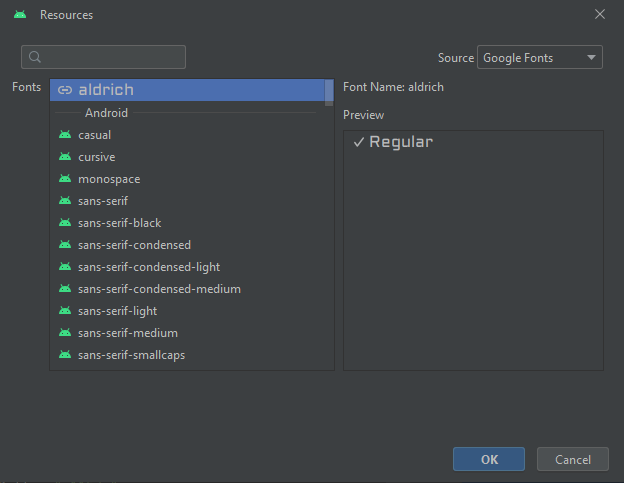
\includegraphics[width=1.0\linewidth]{betutipus}
	\caption{Választott betűtípusom}
	\label{betutipus}
\end{figure}

\section{Layout}
A layout csomag az egyik legmeghatározóbb eleme volt a frontend fejlesztése során. Programom minden Activity fájljához tartozik egy layout is. XML a nyelve ezeknek a fájloknak, mely egy leíró nyelv.

\textit{Alkalmazásom háttérképét ingyenesen töltöttem le, ezen a linken megtekinthető a weboldal: \url{https://www.freepik.com/}}

\subsection{Bejelentkezés}
Az alkalmazásba belépve először a bejelentkezési oldal töltődik be, mely felhasználónevet és jelszót kér az belépéshez. Amennyiben még nincs felhasználói fiók, lehetőség van beregisztrálni is a jelszó alatti szövegre kattintva.

A felhasználónév és jelszó bemeneteit úgy készítettem, hogy egyszerű TextInput helyett létrehoztam egy TextInputLayout-ot, amivel a szövegdoboz tulajdonságait lehet formázni, majd ebben hoztam létre, kihasználva a XML nyelv hierarchiáját, a valódi TextInput-ot, ahová a felhasználó kényelmesen be tudja írni a felhasználónevét és jelszavát.

Külön ikonokat is kerestem a felhasználói élmények javításának érdekében, melyeket a drawable csomagban tárolok. \textit{Az összes ikont, ami nem beépített, erről a weboldalról töltöttem le ingyenesen: \url{https://icons8.com/icons/new}}
\begin{figure}[tbh]
	\centering
	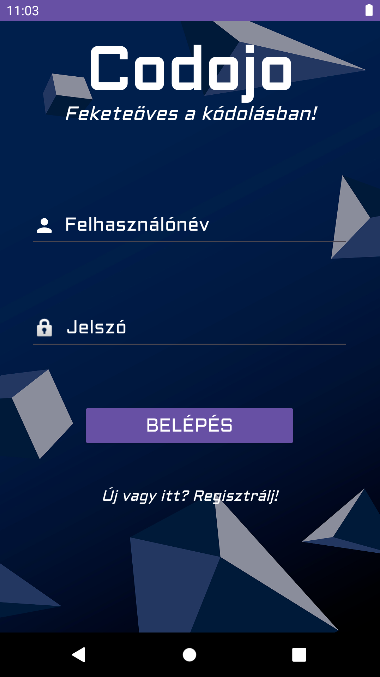
\includegraphics[width=0.55\linewidth]{bejelentkezes}
	\caption{Bejelentkezés layout}
	\label{bejelentkezes}
\end{figure}

\subsection{Regisztráció}
A regisztrációs felület bekéri a felhasználótól a teljes nevét, felhasználónevét, jelszavát és email címét, valamint ha van már a felhasználónak regisztrált fiókja, ebben az esetben biztosítottam a navigálást a bejelentkező felületre. A regisztráció gombra kattintva egyből bejelentkeztet a programba és betölti a főoldalt. Az beviteli adatok megjelenését a bejelentkezés részben leírt módszerrel oldottam meg ennél a résznél is.

Továbbfejlesztési lehetőségként tartom számon azt, hogy megszorításokat adjak meg, hogy a felhasználó például csak 8 karakternél hosszabb jelszót tudjon megadni.
\begin{figure}[tbh]
	\centering
	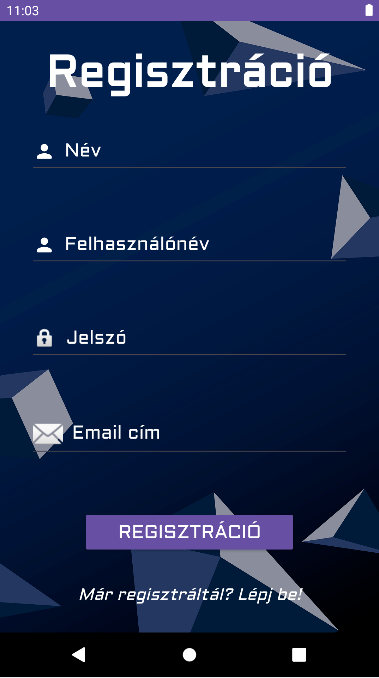
\includegraphics[width=0.6\linewidth]{regisztració}
	\caption{Regisztrációs oldal}
	\label{regisztracio}
\end{figure}

\subsection{Főoldal}
Belépés után a főoldal layout-ja tölt be, melyre egy lelkesítő szöveget írtam, valamint innen érhető el a Profilok, Tanulnivalók, illetve a Kijelentkezés menüpontok. Létrehoztam egy navigációs sávot a menünek, amely az oldal tetején helyezkedik el és Codojo felirat van beillesztve. A sáv jobb oldalán található három darab pont rákattintásával tekinthető meg a menü.

A navigációs sáv elkészítése egy új ,,menu'' nevű csomag létrehozásával járt, amely ugyanabban a mappában helyezkedik el mint például a drawable csomag. Ezen a csomagon belül készítettem egy forrás fájlt, ami tartalmazza a kívánt menüpontokat.

\subsection{Profil}
Felhasználóim a profil menüpontra kattintva megtekinthetik az összes megadott adataikat. Az első és második sorban az aktuális bejelentkezett felhasználó teljes neve, illetve alatta a felhasználóneve jelenik meg, amit a program az adatbázisból tud kiolvasni. Alatta pedig szintén ugyanezek az adatok sorokba rendezve, kiegészítve a jelszóval és email címmel.

Hatékonyabbá úgy tudnám tenni, hogy a jelszót az aktuális jelszó helyett pontokra cserélném, így növelve az adatszivárgás elleni védelmét a programomnak.
\begin{figure}[tbh]
	\centering
	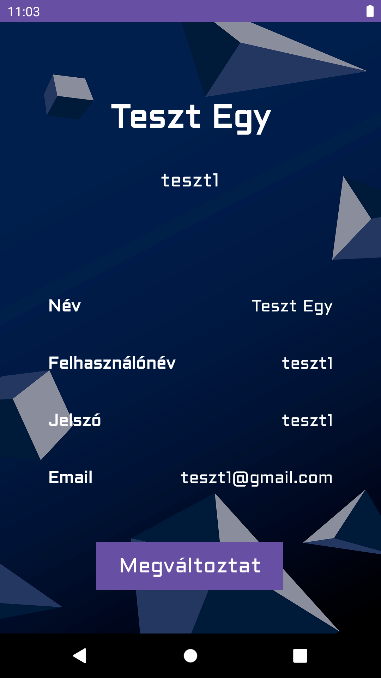
\includegraphics[width=0.4\linewidth]{profil}
	\caption{Profil oldal}
	\label{profil}
\end{figure}
\pagebreak

\subsection{Profiladatok módosítása}
A Profil oldal alján található Megváltoztat gombbal átlépünk arra a felületre, ahol az adott profil adatainak módosítása lehetséges. 

A TextInput mezőkben megjelenik az aktuális adat, amire lehetőség van itt megváltoztatni. A Vissza gombbal visszalépünk a főoldalra, ha mégsem kívánjuk adataink módosítását, a Mentés gombbal pedig elmentjük a változásokat, illetve automatikusan visszaléptet a főoldalra a gomb, amennyiben sikerült a módosítás. Mentés után néhány pillanat múlva frissül a Firebase valós idejű adatbázisa, azonban ahhoz, hogy az applikációban is láthatóak legyenek a változtatások először ki- aztán bejelentkezés szükséges.

\subsection{Tanulnivalók menüpont}
A menüpontra kattintva választhatunk kétféle tananyag közül: Java vagy Python kurzusok. Mindkét anyagrészhez készítettem egy listát, amelyben kiválaszthatjuk, hogy melyiket szeretnénk elolvasni. Külön vannak az egyes fejezethez tartozó kvízek is, egy-egy téma után rögtön kérdésekkel folytatódik a tanulás. A listákat úgy hoztam létre, hogy az egyszerűbbnek vélt témákkal kezdődik és azokkal ér véget, melyekhez egy minimális alaptudás már szükséges. A kvízeket és listákat megkülönböztető ikonokkal láttam el.

Java oldalon a layout fájlban egy olyan View-t használtam, ami lehetővé teszi az oldalon a görgetés funkciót, mely kényelmes használatot biztosít a gomboknak, ennek az osztálynak a neve ScrollView.

\begin{figure}[htb]
	\centering
	\adjustbox{valign=t}{\begin{minipage}[t]{0.45\textwidth}
		\centering
		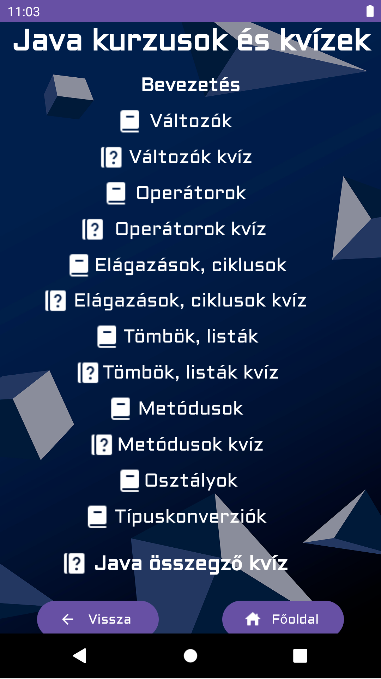
\includegraphics[width=\textwidth]{javalista.png}
		\caption{Java és Python kurzusok listája}
		\label{javalista}
	\end{minipage}}
	\hfill
	\adjustbox{valign=t}{\begin{minipage}[t]{0.45\textwidth}
		\centering
		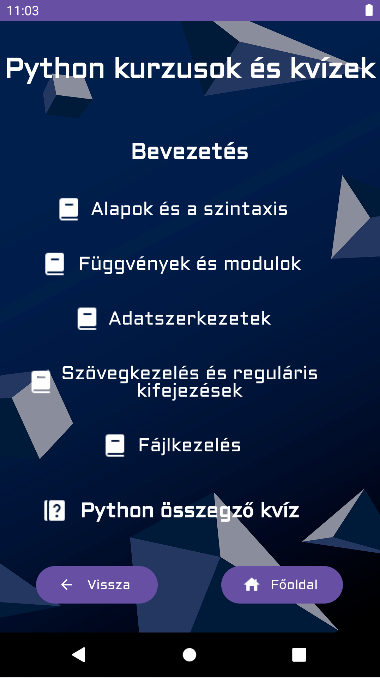
\includegraphics[width=\textwidth]{pythonlista.png}
		\label{pythonlista}
	\end{minipage}}
\end{figure}
\pagebreak
\subsection{Tananyagok}
A kurzusok elkészítésére nagy hangsúlyt fektettem, azért mert ez az egyik legfontosabb része az alkalmazásnak. Előtérbe helyeztem, hogy olvasható legyen a betűtípus, ne túl hosszú legyen a tananyag, hiszen az csökkentheti a felhasználók érdeklődését és figyelmét, illetve átadja a megfelelő alaptudást, annak ellenére, hogy nem hosszú a tananyag. Néhány kurzusba segítségként beillesztettem képeket, ezek saját képek, hogy a felhasználó átfogóbb képet kapjon a témáról.

A tanulnivaló részek alatt létrehoztam navigáló gombokat, melyek biztosítják a kényelmes navigációt a tananyagok és kvízek között, illetve jelzik, hogy melyik témakör vagy kvíz lesz a következő. Ezen gombok bármikor elérhetőek, nem kötöttem feltételekhez használatukat. Minden tananyagot elláttam ScrollView osztállyal biztosítva a megfelelő és kényelmes olvashatóságot

Java és Python kurzusok között mennyiségbeli eltérés van a témák és kvízek tekintetében, melynek oka az, hogy Java nyelven íródott az applikáció. Azonban a program jövőbeni továbbfejlesztésénél a Python témák kibővítését lehetségesnek tartom, mivel fontos, hogy ezt a magas szintű nyelvet is alaposan megismerjék a felhasználók.

A Java tananyagban lévő \textit{explicit}\cite{explicit} és \textit{implicit}\cite{implicit} típuskonverziók képeit az irodalomjegyzékben található weboldalakról töltöttem le.

\begin{figure}[tbh]
	\centering
	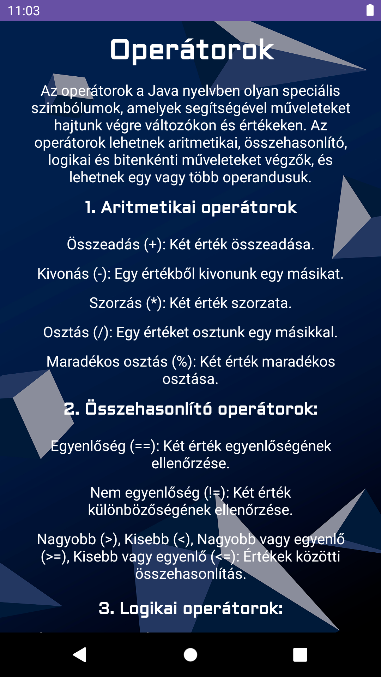
\includegraphics[width=0.6\linewidth]{operatorok}
	\caption{Operátorok téma a Java kurzuson belül}
	\label{operatorok}
\end{figure}

\subsection{Kvízek}
A kvízek megalkotásánál rendkívül nagy figyelmet szenteltem annak, hogy csak olyan kérdést tegyek fel, amire korábban a felhasználó már elolvashatta és megtanulhatta a választ.

A kérdéseket és válaszokat úgy rendeztem el az oldalon, hogy ne okozzon kényelmetlenséget az elolvasásuk. Gombokként definiáltam a válaszokat, amelyből négyféle válaszlehetőség közül lehet kiválasztani a helyes megoldást, mely csak az egyik lehet a négy közül. A kérdéseket úgy állítottam be, hogy ismétlődjenek, azért, mert véleményem szerint ez is nagyban elősegíti a tanulási folyamatot. Tízszer lehet próbálkozni, majd a tizedik kérdés után a teszt ki fogja írni az aktuális tesztben elért pontszámot. Ezután újraindul a teszt, azonban a navigációs gombok segítségével lehetőség van visszalépni a listához vagy továbbhaladni a következő tananyagra.

\begin{figure}[tbh]
	\centering
	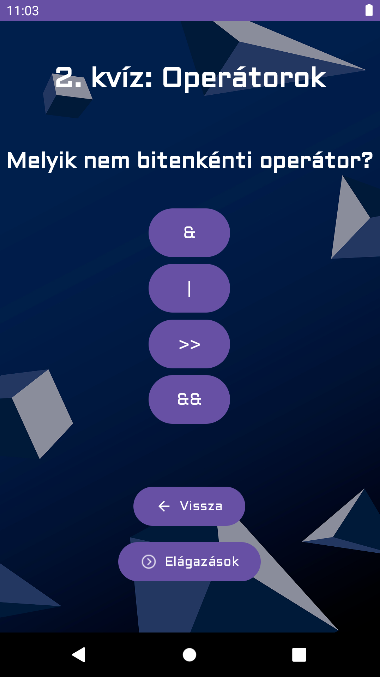
\includegraphics[width=0.6\linewidth]{operatorokkviz}
	\caption{Operátorok téma kvízoldala}
	\label{operatorokkviz}
\end{figure}

\subsection{Kvízek eredményei}
A pontszámot az aktuális teszt végén kiírja a program, valamint a kérdések helyén a próbálkozások számát is. A pontszám alatt lehetőség van a teszt újrapróbálására.

\begin{figure}[tbh]
	\centering
	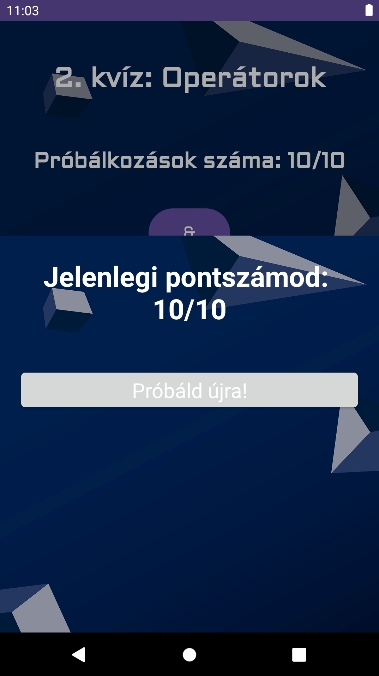
\includegraphics[width=0.7\linewidth]{operatoreredmeny}
	\caption{Eredmények megjelenítése}
	\label{operatoreredmeny}
\end{figure}

\chapter{Az alkalmazás backend fejlesztése}
\section{Regisztráció}
Teljes név, felhasználónév, jelszó és email cím szükséges regisztrációkor a felhasználóknak. Ezt úgy teszem lehetővé, hogy létrehoztam egy üres Activity-t, melynek a XML kódjába belehelyeztem azokat a mezőket, vagyis \textit{TextInputokat}, amelyekbe a felhasználók fogják adataikat beírni. Ezeknek a bemeneteknek egyedi azonosítót (ID) készítettem, majd ezeket az azonosítókat példányosítottam a kapcsolódó osztályban az \textit{onCreate} metóduson belül.

A regisztrációhoz szükségem volt még arra, hogy az adatbázisban is megjelenjenek a beregisztrált adatok. Ehhez a \textit{FirebaseDatabase} és \textit{DatabaseReference} osztályból volt szükségem egy-egy példányra, majd ezeket a regisztráció gombon belül példányosítottam, valamint a \textit{getInstance()} és \textit{getReference()} metódusokat hívtam meg. Előbbi megteremti a kapcsolatot a valós idejű adatbázissal, utóbbi pedig írás és olvasás jogokkal látja el a felhasználót. 

A referencia példánynak meghívtam még két olyan metódusát, melyek segítségével az adatbázisban könnyebben nyomon tudom követni beregisztrált felhasználóim. A \textit{child()} és \textit{setValue()} metódusok meghívása révén beállítottam, hogy a felhasználóneveket jelenítse meg a valós idejű adatbázis közvetlenül a users táblában. Ez megkönnyíti a felhasználók lekövetését, illetve különválasztja egymástól az adatokat.

A bejelentkezéshez és regisztrációhoz készítettem még egy segéd osztályt, melynek \textit{Users} a neve. Ebben konstruktorok, illetve getter és setter metódusok találhatók, amiket a négy adat: teljes név, felhasználónév, jelszó és email mezőkhöz rendeltem hozzá.

Amennyiben sikeres volt regisztrációnk a program kiírja egy üzenetben, hogy sikerült, majd utána bejelentkezéssel együtt a főoldalra navigál. 
\pagebreak
\lstset{
	inputencoding=utf8/latin2,
	language=Java,
	basicstyle=\footnotesize\ttfamily,
	numbers=left,
	breaklines,
	xleftmargin=1.3cm,
	xrightmargin=1.3cm,
	backgroundcolor=\color{gray!30},
	frame=tlbr,
	framesep=2pt,
	keywordstyle=\bfseries\color{blue},
	commentstyle=\itshape\color{red},
	literate={"}{{\textquotedbl}}1
}
\renewcommand{\lstlistingname}{kód}
\lstinputlisting[caption=Regisztráció gomb implementációja,label=regisztracio-java]{regisztracio.java}

\section{Bejelentkezés}
Bejelentkezéshez csupán felhasználónév és jelszó szükséges, melyeket három ellenőrző metódussal egészítettem ki, amik akkor futnak le, ha a felhasználó rákattint a bejelentkezés gombra. 

\subsection{Felhasználónév és jelszó ellenőrzés}
Két \textit{Boolean} típusú függvényt deklaráltam az \textit{onCreate} metóduson kívül, ezekbe pedig egy elágazást implementáltam, mely ellenőrzi, hogy az adott \textit{TextInput} mezője nem-e üres. Az igaz ága akkor teljesül mikor üres a mező, ezután a \textit{setError} eljárást meghívva egy hibaüzenet jelenik meg, miszerint az adott mezőt kötelező kitölteni. Hamis ág esetén a \textit{setError} null értéket ad vissza. 

A jelszó ellenőrző függvényt is ugyanezzel a gondolatmenettel írtam meg.

\lstset{
	inputencoding=utf8/latin2,
	language=Java,
	basicstyle=\footnotesize\ttfamily,
	numbers=left,
	xleftmargin=1.3cm,
	xrightmargin=1.3cm,
	backgroundcolor=\color{gray!30},
	framesep=2pt,
	keywordstyle=\bfseries\color{blue},
	commentstyle=\itshape\color{red},
	literate={"}{{\textquotedbl}}1
}
\renewcommand{\lstlistingname}{kód}
\lstinputlisting[caption=A felhasználónév ellenőrző függvénye,label=bejelentkezes-felhasznalonev]{bejelentkezesfelhasznalonev.java}

\subsection{Regisztrált felhasználó ellenőrzése}
\label{Regisztrált felhasználó ellenőrzése}
A bejelentkezés elengedhetetlen része, hogy csak azokat a felhasználókat engedje bejelentkezni, akik előtte már beregisztráltak. Ehhez egy eljárást írtam, melynek a neve \textit{checkUser}. 

Szükségem volt ebben az eljárásban is a \textit{DatabaseReference} osztályból egy mezőre, melyhez hozzárendeltem a \textit{FirebaseDatabase} osztály \textit{getInstance()} és \textit{getReference()} metódusát, melyek az adatbázis eléréséért felelnek. Majd a \textit{Query} osztályú változóhoz kapcsoltam hozzá az előbb létrehozott mezőt, mely a felhasználónévre rendezetten egy keresést hajt végre, ahol a \textit{username} mező megegyezik az eljárásban deklarált \textit{user} változóval.

\lstset{
	inputencoding=utf8/latin2,
	language=Java,
	basicstyle=\footnotesize\ttfamily,
	numbers=left,
	xleftmargin=1.7cm,
	xrightmargin=1.7cm,
	backgroundcolor=\color{gray!30},
	framesep=2pt,
	keywordstyle=\bfseries\color{blue},
	commentstyle=\itshape\color{red},
	literate={"}{{\textquotedbl}}1
}
\renewcommand{\lstlistingname}{kód}
\lstinputlisting[caption=Adatbázishoz való kapcsolódás,label=query]{query.java}

Ezután meghívtam az \textit{addListenerForSingleValueEvent} metódust, mely egyszeri alkalommal lekérdezi az adatokat a valós idejű adatbázisból. Automatikusan meghívásra kerül egy sikeres és egy sikertelen lekérdezésre vonatkozó eljárás, melyek \textit{DataSnapshot} típusúként kezelik a lekért adatokat. Az első elágazásban ellenőrzöm, hogy van-e regisztrált felhasználó és az igaz ágában beállítok egy \textit{setError} üzenetet nulla értékűre, hiszen talált regisztrált felhasználót, valamint kinyerem az adatbázisban tárolt jelszót és elmentem egy új változóba.

Ezt követően egy második elágazásban ellenőrzöm, hogy a bejelentkezéshez használt jelszó egyezik-e az adatbázisban tárolt jelszóval. A teljes név, felhasználónév, jelszó és email cím mezőket kiolvasom az adatbázisból és elmentem egy új változóba. Majd ezeket a \textit{SharedPreferences} interfész segítségével tárolom, mely kulcs-értékként kezeli az adatokat. Mindezek után a program átnavigál a főoldalra, amennyiben nem került egyik hamis ágba sem.

\lstset{
	inputencoding=utf8/latin2,
	language=Java,
	basicstyle=\footnotesize\ttfamily,
	numbers=left,	
	xleftmargin=0.5cm,
	xrightmargin=0.5cm,
	backgroundcolor=\color{gray!30},
	framesep=2pt,
	keywordstyle=\bfseries\color{blue},
	commentstyle=\itshape\color{red},
	literate={"}{{\textquotedbl}}1
}
\renewcommand{\lstlistingname}{kód}
\lstinputlisting[caption=A regisztrált felhasználók ellenőrzése,label=felhasznalo]{felhasznalo.java}

\section{Profil}
Ezen oldalon a felhasználó ellenőrizni tudja, hogy milyen adatokat adott meg regisztrációkor, ezek az adatok vannak jelen az adatbázisban is. Valamint erről az oldalról tud átlépni arra a felületre, ahol ezeket módosítani tudja.

Egy \textit{Data()} és egy \textit{Check()} nevű eljárást készítettem, hogy mindezeket lehetővé tegye. A két eljárás meghívását az \textit{onCreate} metódus törzsébe helyeztem.

\subsubsection{Data}
Ebben az eljárásban a korábban létrehozott regisztrációs adatokat, melyeket a \textit{SharedPreferences} interfész segítségével tárolom, először kiolvasom az adatbázisból, majd pedig ezeket beállítom a \textit{TextInputok} helyére. 

\subsubsection{Check}
Ezt az eljárást hasonlóan írtam meg, mint az \ref{Regisztrált felhasználó ellenőrzése} fejezetben lévő metódust. A különbség, hogy ezen az oldalon csak az adatok megjelenítésére fókuszáltam, így nem kellett kulcs-érték párokat létrehoznom és tárolnom a \textit{SharedPreferences} segítségével, valamint a felhasználó négy megadott adatát Intent típussá konvertálja és átküldi arra az oldalra, ahol ezeket már módosítani is tudja.

Lefutni akkor fog, mikor a felhasználó rákattint a \textit{Megváltoztat} gombra, ezzel elnavigálja a profil módosítására szolgáló oldalra.

\section{Profil módosítása}
Az oldalt úgy állítottam be, hogy a felhasználó ezen az oldalon is megtekinthesse a módosítandó adatait. Ehhez megírtam a \textit{DataChange()} nevű eljárást, mely az előző oldalról átküldött adatokat beállítja a megfelelő bemeneti helyekre.

Három ellenőrző, \textit{boolean} típusú függvényt írtam a felhasználónév, jelszó és email cím módosításához. Úgy működnek, hogy először összehasonlítja az eltárolt adatokat az új adatokkal, majd utána az adatbázisban tárolt régi adatot frissíti az újra. 

Mindhárom függvényt a Mentés gomb implementációjába építettem bele. Egy elágazás megvizsgálja, hogy sikeresen lefutott-e, ehhez \textit{VAGY} operátort használtam azért, mert egyszerre nem biztos, hogy mindegyik adatot szeretné módosítani a felhasználó. Ezután amennyiben sikerült a változtatás egy üzenet jön a sikerességről, illetve átnavigál a program a főoldalra.

\lstset{
	inputencoding=utf8/latin2,
	language=Java,
	basicstyle=\footnotesize\ttfamily,
	numbers=left,	
	xleftmargin=0.5cm,
	xrightmargin=0.5cm,
	backgroundcolor=\color{gray!30},
	framesep=2pt,
	keywordstyle=\bfseries\color{blue},
	commentstyle=\itshape\color{red},
	literate={"}{{\textquotedbl}}1
}
\renewcommand{\lstlistingname}{kód}
\lstinputlisting[caption=Jelszó megváltoztatásának függvénye,label=jelszo]{jelszo.java}

Módosítani jelenleg csak három adatot tud a felhasználó, továbbfejlesztési ötletként tartom számon a felhasználónév módosítását.

\section{Főoldal}
Ezen az oldalon található a saját navigációs sávom, melynek profil, tanulnivalók és kijelentkezés menüpontokkal készítettem el. A menü navigációját egy switch-case-zel oldottam meg az \textit{onOptionsItemSelected} boolean típusú függvényen belül, valamint a kijelentkezés opcióban implementáltam \textit{FirebaseAuth} osztály egy változóját, melyet elláttam a \textit{signOut()} metódussal, mely az adatbázisból való kijelentkezést végzi.

\section{Kvízek}
A tanulnivalók menüpontra kattintva tekinthetjük meg az oldalt, ahol kétféle kvíz közül választhatunk. Ezeket egy-egy gomb implementálásával készítettem el, melyek elkalauzolnak a választott kurzus tananyagainak listájához. 

\subsection{Kurzuslisták}
A Java és Python tananyagok listáival az volt a célom, hogy biztosítsam a felhasználónak azt az élményt, hogy előre megtekintse milyen témák várhatóak a kurzus során, illetve, hogy mennyire gyakran fog találkozni számon kérő kérdésekkel. A Java lista esetében, mely sokkal több témát dolgoz fel mint a Python, görgethetővé kellett tennem, melyben a \textit{ScrollView} osztály volt a segítségemre. A listákban található kurzusokat \textit{TextView}-ként implementáltam, majd deklarálás és inicializálás után mindegyikhez meghívtam a \textit{setOnClickListener} metódust, mely navigációt biztosít a választott kurzushoz.

\subsection{Kurzusok oldalai}
Az összes oldal aljára navigáló gombokat helyeztem, amelyek közül az egyik visszavisz a választott kurzus témáinak listájához, másik pedig a soron következő kvíz vagy tananyag oldalára navigál át.

\subsection{Kvízek felépítése}
Négy válaszlehetőséggel készítettem el a kvízeket, melyeknek az a lényege, hogy a felhasználói felületen, mikor kiválaszt egy lehetséges megoldást a felhasználó, akkor ezt leellenőrzik, majd eltárolják metódusok, valamint ha helyes volt a válasz akkor növelik a pontszámot és véletlenszerűen választanak egy következő kérdést.

A kérdések és válaszok elkészítése előtt szükségem volt egy olyan segédosztályra, melyben konstruktorok, getter és setter metódusok találhatók, a programomban ez az osztály a \textit{Quizzes}. 

A válaszlehetőségeket gombokkal implementáltam, majd ezeknek \textit{setOnClickListener} metódusába építettem bele az ellenőrzést, pontszám és próbálkozások számának növelését, valamint az új kérdés pozíciójának a lekérdezését, majd megjelenítését.

\lstset{
	inputencoding=utf8/latin2,
	language=Java,
	basicstyle=\footnotesize\ttfamily,
	numbers=left,	
	xleftmargin=0.5cm,
	xrightmargin=0.5cm,
	backgroundcolor=\color{gray!30},
	framesep=2pt,
	keywordstyle=\bfseries\color{blue},
	commentstyle=\itshape\color{red},
	literate={"}{{\textquotedbl}}1
}
\renewcommand{\lstlistingname}{kód}
\lstinputlisting[caption=Válaszlehetőség ellenőrzésének a kódja,label=kviz]{kviz.java}

Három privát eljárásra is szükségem volt, melyek más-más a szerepük.
\subsubsection{Pontszám megjelenítése}
A pontszámot kvíz végén vagyis a tizedik próbálkozás után fogja megjeleníteni a program, továbbá egy gomb segítségével újra meg lehet próbálni a kérdéssorozatot.

\subsubsection{Kérdések megjelenítése}
Ebben a metódusban egy elágazás ellenőrzi, hogy megvolt-e a tizedik próbálkozás is, amennyiben igen, meghívja a pontszámok megjelenítéséhez használt eljárást, ha pedig még nem, akkor megjeleníti a kérdést és a hozzá tartozó válaszokat.

\subsubsection{Kérdések hozzáadása}
Egy előre deklarált listába gyűjtöm össze ebben az eljárásban a kérdéseket az \textit{add()} segítségével. Paraméterlistába \textit{Quizzes} típust tettem, mivel így hozzá tudom adni rögtön a kérdést, a négy válaszlehetőséget és a megoldást.

\chapter{Tesztelés}
Applikációm teszteléséhez a Firebase beépített modulját, a Test Lab-et választottam, mellyel egyszerűen, de nagy hatékonysággal lehet letesztelni a program funkcióit. A Test Lab többféle tesztelési funkciót felajánlott számomra, azonban a Robo tesztekre esett a választásom, melynek automatizált tesztelési rendszere van, amihez nem kell külön programot írni. Az automatikus tesztek mellett manuális teszteket is végeztem, melyek megfelelő visszajelzéseket adtak programom fejlesztés közben.

\section{Test Lab}
A tesztek létrehozásához először szükségem volt arra, hogy felismerje a programomat és az adatbázis a Test Lab. Emiatt készítenem kellett egy .apk kiterjesztésű fájlt, melyet a gradle biztosít. Ehhez először meg kellett tisztítanom a kódot a \textit{Clean Project} paranccsal, melyet a Build menüpontban érek el. Ezután pedig a gradle fájlban létre kellett hoznom a .apk kiterjesztésű fájlt a \textit{Build APK} parancs segítségével.

Ezekre az előkészületekre azért volt szükség, mivel az APK kiterjesztésű fájl biztosítja a kapcsolatot a programom, továbbá az adatbázis és a Test Lab között. A következő lépésben határozzuk meg, hogy milyen tesztet szeretnénk elindítani.

\section{Robo tesztek}
Ehhez a fajta tesztekhez szükségem volt az előkészületekben megtett lépéseimre, melynek eredménye az APK típusú fájl, ami a teszt fajtájának kiválasztása után fel kell tölteni a megadott helyre. Ezután lehetőség nyílik egy eszközt választani, melyen majd a tesztelés fog futni. Virtuális és fizikai eszközök széles választékából lehet kiválasztani a tesztelésre hivatott telefont vagy tabletet.

A program futtatásához Android Studioban én egy 30-as API szintű készüléket használtam, amelyen hiba nélkül lefutott minden funkciója, ezért a tesztelésnél ki szerettem volna próbálni másfajta API szintű eszközöket is, ezért elsősorban egy Galaxy S20 készülékre esett a választásom, mely 29-es API szintű, azaz Android 10 operációs rendszer van rajta. A szintek, valamint a verziók megtekinthetőek az \ref{apiszintek} ábrán.

Miután kiválasztásra került az eszköz, a további opcióknál be lehet állítani, hogy milyen adatokkal jelentkezzen be a teszthez. Ezért készítettem egy teszt fiókot, mely a teszt2 felhasználónevet kapta, ugyanezzel a jelszóval. Ezután be kell állítani azt az azonosítót, ahova ezt az értéket fogja beírni, vagyis azt a \textit{TextInput} ID-t, amit a programban is használok. Valamint hozzá lehet adni gombokat, további bemeneteket, ha szükség van rá és azt is, hogy mit ne vizsgáljon meg a teszt során. A bejelentkezést teszteltem, mely sikeresen lefutott több készüléken. Az egyik Galaxy S20, a másik pedig Galaxy S22 Ultra készüléken teszteltem.

\begin{figure}[tbh]
	\centering
	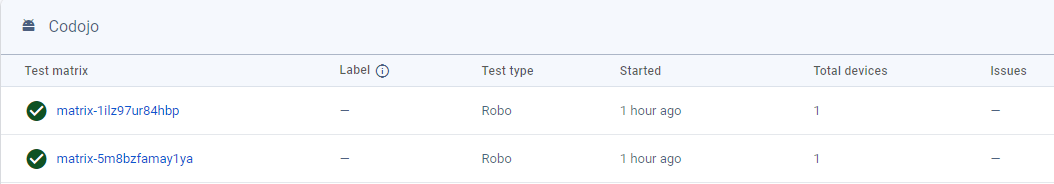
\includegraphics[width=1.0\linewidth]{teszteles}
	\caption{Sikeres Robo tesztek listája}
	\label{teszteles}
\end{figure}

\section{Manuális tesztek}
Manuális tesztelést főleg a bejelentkezés, regisztráció, módosítás és kijelentkezés funkcióknál, valamint a kvízek pontszámainál használtam.

\begin{tabular}{|p{2cm}|p{9cm}|p{3cm}|}
	\hline
	\multicolumn{1}{|c|}{Azonosító} & \multicolumn{1}{c|}{Funkció} & \multicolumn{1}{c|}{Állapot} \\
	\hline
	\multicolumn{1}{|c|}{Regisztráció} & A regisztráció gombra kattintva a bemeneti adatok ellenőrzése metódusok által, valamint a valós idejű adatbázisba való feltöltés & \multicolumn{1}{c|}{Sikeres} \\
	\hline
	\multicolumn{1}{|c|}{Bejelentkezés} & A bejelentkezés gombra kattintással a megadott felhasználónév és jelszó páros ellenőrzése és összehasonlítása az adatbázis tárolt értékkel, majd a főoldal betöltése & \multicolumn{1}{c|}{Sikeres}  \\
	\hline
	\multicolumn{1}{|c|}{Profil} & A regisztrációhoz megadott adatok kiolvasása az adatbázisból, majd ezek megjelenítése a felhasználó számára & \multicolumn{1}{c|}{Sikeres}  \\
	\hline
	\multicolumn{1}{|c|}{Profil módosítása} & A beregisztrált adatok kiolvasása az adatbázisból és módosítása, majd ezen változtatások frissítése az adatbázisban & \multicolumn{1}{c|}{Sikeres}  \\
	\hline
	\multicolumn{1}{|c|}{Kvízek} & A kérdések és válaszok megjelenítése és kinyerése listából. & \multicolumn{1}{c|}{Sikeres}  \\
	\hline
	\multicolumn{1}{|c|}{Pontszám} & A helyes megoldások után a pontszám és a próbálkozások számának növelése, 10 próbálkozás után eredmény kiírása. & \multicolumn{1}{c|}{Sikeres}  \\
	\hline
	\multicolumn{1}{|c|}{Kijelentkezés} & A gombra kattintva a felhasználó kijelentkeztetése. & \multicolumn{1}{c|}{Sikeres}  \\
	\hline
\end{tabular}
\chapter*{Összegzés}
Szakdolgozatomban részletesen bemutattam azon technológiákat, valamint a frontend és backend fejlesztését, illetve az applikáció tesztjeit. Szorosan kapcsolódó témákat, mint például az informatikaoktatást, továbbá napjainkat érintő változásokat és problémákat az iparban is érintettem.

A programom továbbfejlesztése is nagyban foglalkoztat, hiszen szeretném még hatékonyabbá tenni leendő felhasználóim tanulási élményeit. 

További ellenőrző metódusokat vezetnék be a bejelentkezés és regisztráció felületekre, amik ellenőrzik például, hogy 8 karakternél többet írt-e a jelszóhoz a felhasználó, amennyiben nem, úgy hibát talál és figyelmeztet, hogy nem felel meg a begépelt jelszó a megadott kritériumoknak.

Frontend tekintetében a a menüpontokat úgy alakítanám át, hogy egy teljesen új \textit{NavigationDrawer-t} írnék, melyben a menü nem lenyíló lenne, hanem oldalsávos, mely addig rejtve van, amíg a felhasználó rá nem kattint a megfelelő ikonra.

A profil oldalt kiegészíteném egy profilképpel, melyet a felhasználó feltölthet vagy választhat az előre feltöltött képekből, valamint ezt a profilon meg is jelenítené, a módosítás oldalon pedig meg tudná változtatni.

A kvízek tekintetében pontrendszert vezetnék be, amely az adatbázissal áll kapcsolatban és tárolja a felhasználók pontszámait. A kvízeket még több kérdéssel, illetve egy előrehaladást megjelenítő sávval látnám még el.

A felhasználói élményeket fokozva egy jutalomrendszer is bevezetnék, mely biztatja a felhasználót a továbbhaladásra, valamint ösztönzi a kvízek kitöltésére. Ha a felhasználó elért egy bizonyos százalékot minden egyes kvízben, további plusz anyagokat tennék számára elérhetővé, melyben akár ki is próbálhatná a programozást az applikációban.

	\begin{thebibliography}{14}
		\setlength{\itemindent}{0em}
		\bibitem{android_studio} \textsc{Android Studio: \url{https://developer.android.com/studio/intro}}
		\bibitem{firebase} \textsc{Firebase: \url{https://www.geeksforgeeks.org/firebase-introduction/}}
		\bibitem{firebase_realtime} \textsc{Firebase Realtime Database: \url{https://firebase.google.com/docs/database}}
		\bibitem{firebase_auth} \textsc{Firebase Authentication: \url{https://crane.hu/amit-a-google-firebase-rol-tudni-erdemes}}
		\bibitem{github} \textsc{GitHub: \url{https://hub.hellowp.io/docs/tudasbazis/oktatoanyagok/github/github-kezdoknek/}}
		\bibitem{api} \textsc{API: \url{https://apilevels.com/}}
		\bibitem{java} \textsc{Java: \url{https://azure.microsoft.com/hu-hu/resources/cloud-computing-dictionary/what-is-java-programming-language}}
		\bibitem{gitkraken} \textsc{GitKraken: \url{https://dev.to/iphytech/gitkraken-what-is-it-and-common-actions-5531}}
		\bibitem{informatika_oktatas} \textsc{Informatika oktatás Magyarországon: \url{https://www.speaknyelviskola.hu/milyen-a-jelenlegi-informatikuskepzes-magyarorszagon/}}
		\bibitem{bootcamp} \textsc{Bootcamp: \url{https://24.hu/tech/2024/03/07/it-szektor-programozo-szamitogepes-szakember-hiany-bootcamp-bezaras/}}
		\bibitem{krizis} \textsc{Krízishelyzet: \url{https://telex.hu/techtud/2024/02/23/techcegek-it-leepites-kirugas-ai-covid-microsoft-google-amazon-apple-meta}}
		\bibitem{palyakezdok} \textsc{Pályakezdők helyzete: \url{https://telex.hu/gazdasag/2024/03/07/perelnek-a-tanulok-akiket-cserben-hagyott-a-biztos-elhelyezkedest-igero-programozosuli?fbclid=IwAR3Nrs9MhEzP_qY4xYGXlCrKlgQyGM0qlUW9vEQDKmzHiLTJd2771TKpxio}}
		\bibitem{explicit} \textsc{Explicit: \url{https://www.geeksforgeeks.org/typecasting-in-java/}}
		\bibitem{implicit} \textsc{Implicit: \url{https://techvidvan.com/tutorials/java-type-conversion/}}
	\end{thebibliography}
\end{document}